\documentclass[12pt]{article}
\usepackage[russian]{babel}
\usepackage{geometry}

\usepackage{graphicx} % вставка изображений
\usepackage{caption} % описание изображений

%различные цветовые модели
\usepackage[usenames]{color}
\usepackage[dvipsnames,table]{xcolor}
\usepackage{colortbl}

\usepackage{tikz}
\usetikzlibrary{shapes, arrows}
\usepackage{varwidth}
\usepackage{ifthen}

\usepackage{multicol} % вставка изображений в две колонки


%циклы foreach в tikz и создание переменных внутри этого окружения
\usepackage{pgffor}
\usepackage{pgfmath}

\usepackage{xifthen}

\usepackage{afterpage}

\usepackage{amssymb}
\usepackage{amsmath}

\usepackage{hyperref}

\usepackage[utf8]{inputenc}

\tikzstyle{connector} = [draw, -latex']
\tikzstyle{line} = [draw, -]
\tikzstyle{dashed} = [draw, -, dash pattern=on 5pt off 5pt]


\usepackage{listings}
\usepackage{listingsutf8}
\usepackage[T2A]{fontenc}
\newcommand{\listingsttfamily}{\usefont{T2A}{PTMono-TLF}{m}{n}}

\lstset{
	language=C,                % choose the language of the code
	numbers=left,                   % where to put the line-numbers
	stepnumber=1,                   % the step between two line-numbers.        
	numbersep=5pt,                  % how far the line-numbers are from the code
	backgroundcolor=\color{black},  % choose the background color. You must add \usepackage{color}
	commentstyle=\color{Gray},
	basicstyle=\listingsttfamily\color{Gray},
	keywordstyle=\color{BurntOrange},
	stringstyle=\color{YellowGreen},
	showspaces=false,               % show spaces adding particular underscores
	showstringspaces=false,         % underline spaces within strings
	showtabs=false,                 % show tabs within strings adding particular underscores
	tabsize=4,                      % sets default tabsize to 2 spaces
	captionpos=b,                   % sets the caption-position to bottom
	breaklines=true,                % sets automatic line breaking
	breakatwhitespace=true,         % sets if automatic breaks should only happen at whitespace
	title=\lstname, 
	inputencoding=utf8,                % show the filename of files included with \lstinputlisting;
	extendedchars=\true,
	keepspaces=true
}

\geometry{top=2cm, bottom=2cm, left=3cm, right=1.5cm}
\textheight=24cm
\textwidth=18cm
\flushbottom 

\oddsidemargin=0pt 
\topmargin=-1.5cm 
\parskip=0.25cm
\parindent=24pt 

\tolerance=2000 

\setcounter{secnumdepth}{0}

\begin{document}
	\begin{center}
		{\parskip=1cm
			МИНИСТЕРСТВО НАУКИ И ВЫСШЕГО ОБРАЗОВАНИЯ РОССИЙСКОЙ ФЕДЕРАЦИИ
			
			ФЕДЕРАЛЬНОЕ ГОСУДАРСТВЕННОЕ БЮДЖЕТНОЕ ОБРАЗОВАТЕЛЬНОЕ УЧРЕЖДЕНИЕ ВЫСШЕГО ОБРАЗОВАНИЯ
			
			{\bf«БЕЛГОРОДСКИЙ ГОСУДАРСТВЕННЫЙ ТЕХНОЛОГИЧЕСКИЙ УНИВЕРСИТЕТ им. В. Г. Шухова»\\(БГТУ им. В. Г. Шухова)}
			
			\begin{figure}[bh]
				\noindent\centering{
					
\includegraphics[width=100mm]{images/start_logo.png}
					\captionsetup{labelformat=empty}
				}
			\end{figure}
			Кафедра программного обеспечения вычислительной техники и автоматизированных систем
		}
		
		{\Large 
			\vspace{1cm}
			{\parskip=0.25cm 
				{\bf Лабораторная работа №3.1}
				
				по дисциплине: «Дискретная математика»

				по теме: {\bf Отношения и их свойства}
			}
		}
	\end{center}	
	\begin{flushleft}
		{\leftskip=10cm
			{\vspace{3cm} Выполнил/a: ст. группы ПВ-231}
			
			Чупахина София Александровна
			
			Проверил: Рязанов Юрий Дмитриевич
			
		}
	\end{flushleft}
	\begin{center}
		{\parskip=3cm Белгород, 2024}
	\end{center}
	\newpage
	
	\tableofcontents
	\newpage
	
	\section{Часть 1. Операции над отношениями}
	\label{startpart1}
	{\bf Вариант 6} 
	\begin{description}
		\item[а)] $A = \{(x, y)$ | $x + y$ --- четно и $x + y > 8\}$ \\
		$B = \{(x, y)$ | $x + 2y > 20\}$ \\
		$C = \{(x, y)$ | $(x, y) \in \{1, 2, 4, 8\} \times \{3, 5, 7, 10\} \}$
		\item[б)] D = $A \cap B^{-1} \bigtriangleup A o B o C$
	\end{description}
	\subsection{Задание 1.1}
	\label{subpart1_1}
	{\bf Текст задания:} представить заданные на множестве $M = \{1, 2, 3, 4, 5, 6, 7, 8, 9, 10\}$ отношения $A, B, C$ графиком, графом и матрицей.
	
	Начнем с отношения $A$. На графике (первой четверти координатной плоскости с координатами, не превышающими 10) элементам отношения будут соответствовать точки, находящиеся строго выше линии $y = 8 - x$ (для удобства обозначим ее на графике пунктиром), сумма координат которых при этом четна.
	
	\begin{tikzpicture}{line width=3pt}
	\draw[step=0.75] (0,0) grid (7.5, 7.5);
	\draw[-latex', line width=3pt] (0, 0) -- (0, 8.25);
	\draw[-latex', line width=3pt] (0, 0) -- (8.25, 0);
	
	\foreach \x in {1, 2,...,10} {
		\draw (-0.5, 0.75*\x) node{\x};
		\draw (0.75*\x, -0.5) node{\x};
	};
	
	\foreach \x in {1, 2,...,10} {
		\foreach \y in {1, 2,...,10} {
			\pgfmathparse{ifthenelse(\x + \y > 8, ifthenelse(Mod(\y + \x, 2) == 0, 1, 0), 0};
			\ifodd\pgfmathresult\relax
			\fill[red] (0.75*\x, 0.75*\y) circle (3pt);
			\fi
		}
	};
	\draw[dashed] (0, 6) -- (6, 0);
	\end{tikzpicture}
	
	С помощью графа это отношение можно представить следующим образом. Отдельно можно заметить, что, поскольку вхождение или невхождение элемента в отношение определяется только суммой координат, при соответствующих условиям $x$ и $y$ элементом отношения будет являться как $(x, y)$, так и $(y, x)$, а потому граф состоит только из ребер.
	
	\newpage
	
		\begin{tikzpicture}
		\def\radius{4} % Радиус внешнего круга
		\def\numcircles{10} % Количество внутренних кругов
		\foreach \i in {1,...,\numcircles} {
			\pgfmathsetmacro\angle{360*\i/\numcircles} % Угол для текущего круга
			\pgfmathsetmacro\x{\radius*cos(\angle)} % Координата x центра круга
			\pgfmathsetmacro\y{\radius*sin(\angle)} % Координата y центра круга
			\node[circle, draw=black, minimum height=1cm] at (\x, \y) (knot\i) {\i};
		};
		
		\foreach \x in {1,...,\numcircles} {
			\foreach \y in {1,...,\numcircles} {
				\pgfmathparse{ifthenelse(\x + \y > 8, ifthenelse(Mod(\y + \x, 2) == 0, 1, 0), 0};
				\ifodd\pgfmathresult\relax
				\pgfmathparse{ifthenelse(\y == \x, 1, 0};
				\ifodd\pgfmathresult\relax
				\pgfmathsetmacro\angle{360*\x/\numcircles}; % Угол для текущего круга
				\pgfmathsetmacro\xcoord{\radius*cos(\angle)}; % Координата x центра круга
				\pgfmathsetmacro\ycoord{\radius*sin(\angle)}; % Координата y центра круга
				\pgfmathsetmacro\xshift{1.5*cos(90 - \angle)}; % Координата x центра круга
				\pgfmathsetmacro\yshift{1.5*cos(\angle)}; % Координата x центра круга
				\path[line, line width = 1.5pt] (knot\x) .. controls (\xcoord*1.5 - \xshift, \ycoord*1.5 + \yshift) and (\xcoord*1.5 + \xshift, \ycoord*1.5 - \yshift) .. (knot\y);
				\else
				\path[line, line width = 1.5pt] (knot\x) -- (knot\y);	
				\fi						
				\fi
			};
		};
	\end{tikzpicture}
	
	В виде матрицы же отношение $A$ будет представлено следующим образом. Тут можно заметить, что единицы в матрице не совпадают с расположением точек графика: чтобы они совпали, график нужно мысленно повернуть на 90$^{\circ}$ по часовой стрелке:
	
	\begin{tabular} {c c c c c c c c c c}
		0 & 0 & 0 & 0 & 0 & 0 & 0 & 0 & 1 & 0 \\
		0 & 0 & 0 & 0 & 0 & 0 & 0 & 1 & 0 & 1 \\
		0 & 0 & 0 & 0 & 0 & 0 & 1 & 0 & 1 & 0 \\
		0 & 0 & 0 & 0 & 0 & 1 & 0 & 1 & 0 & 1 \\
		0 & 0 & 0 & 0 & 1 & 0 & 1 & 0 & 1 & 0 \\
		0 & 0 & 0 & 1 & 0 & 1 & 0 & 1 & 0 & 1 \\
		0 & 0 & 1 & 0 & 1 & 0 & 1 & 0 & 1 & 0 \\
		0 & 1 & 0 & 1 & 0 & 1 & 0 & 1 & 0 & 1 \\
		1 & 0 & 1 & 0 & 1 & 0 & 1 & 0 & 1 & 0 \\
		0 & 1 & 0 & 1 & 0 & 1 & 0 & 1 & 0 & 1 \\
	\end{tabular}
	
	Перейдем к отношению $B$. На графике элементам отношения будут соответствовать точки, находящиеся строго выше линии $y = 10 - 0.5x$ (для удобства также обозначим ее на графике пунктиром).
	
	\begin{tikzpicture}{line width=3pt}
	\draw[step=0.75] (0,0) grid (7.5, 7.5);
	\draw[-latex', line width=3pt] (0, 0) -- (0, 8.25);
	\draw[-latex', line width=3pt] (0, 0) -- (8.25, 0);
	
	\foreach \x in {1, 2,...,10} {
		\draw (-0.5, 0.75*\x) node{\x};
		\draw (0.75*\x, -0.5) node{\x};
	};
	
	\foreach \x in {1, 2,...,10} {
		\foreach \y in {1, 2,...,10} {
			\pgfmathparse{ifthenelse(\x + 2*\y > 20, 1, 0};
			\ifodd\pgfmathresult\relax
			\fill[red] (0.75*\x, 0.75*\y) circle (3pt);
			\fi
		}
	};
	\draw[dashed] (0, 7.5) -- (7.5, 3.75);
	\end{tikzpicture}
	
	С помощью графа это отношение можно представить следующим образом. В отличие от предыдущего отношения, на этом графе присутствуют как ребра, так и дуги.
	
	\begin{tikzpicture}
		\def\radius{4} % Радиус внешнего круга
		\def\numcircles{10} % Количество внутренних кругов
		\foreach \i in {1,...,\numcircles} {
			\pgfmathsetmacro\angle{360*\i/\numcircles} % Угол для текущего круга
			\pgfmathsetmacro\x{\radius*cos(\angle)} % Координата x центра круга
			\pgfmathsetmacro\y{\radius*sin(\angle)} % Координата y центра круга
			\node[circle, draw=black, minimum height=1cm] at (\x, \y) (knot\i) {\i};
		};
		
		\foreach \x in {1,...,\numcircles} {
			\foreach \y in {1,...,\numcircles} {
				\pgfmathparse{ifthenelse(\x + 2*\y > 20, 1, 0};
				\ifodd\pgfmathresult\relax
				\pgfmathparse{ifthenelse(\y == \x, 1, 0};
				\ifodd\pgfmathresult\relax
				\pgfmathsetmacro\angle{360*\x/\numcircles}; % Угол для текущего круга
				\pgfmathsetmacro\xcoord{\radius*cos(\angle)}; % Координата x центра круга
				\pgfmathsetmacro\ycoord{\radius*sin(\angle)}; % Координата y центра круга
				\pgfmathsetmacro\xshift{1.5*cos(90 - \angle)}; % Координата x центра круга
				\pgfmathsetmacro\yshift{1.5*cos(\angle)}; % Координата x центра круга
				\path[line, line width = 1.5pt] (knot\x) .. controls (\xcoord*1.5 - \xshift, \ycoord*1.5 + \yshift) and (\xcoord*1.5 + \xshift, \ycoord*1.5 - \yshift) .. (knot\y);
				\else
				\pgfmathparse{ifthenelse(\y + 2*\x > 20, 1, 0};
				\ifodd\pgfmathresult\relax
				\path[line, line width = 1.5pt] (knot\x) -- (knot\y);
				\else
				\path[connector, line width = 1.5pt] (knot\x) -- (knot\y);	
				\fi
				\fi						
				\fi
			};
		};
	\end{tikzpicture}
	
	Матрица, представляющая это отношение, будет выглядеть следующим образом:
	
	\begin{tabular} {c c c c c c c c c c}
		0 & 0 & 0 & 0 & 0 & 0 & 0 & 0 & 0 & 1 \\
		0 & 0 & 0 & 0 & 0 & 0 & 0 & 0 & 0 & 1 \\
		0 & 0 & 0 & 0 & 0 & 0 & 0 & 0 & 1 & 1 \\
		0 & 0 & 0 & 0 & 0 & 0 & 0 & 0 & 1 & 1 \\
		0 & 0 & 0 & 0 & 0 & 0 & 0 & 1 & 1 & 1 \\
		0 & 0 & 0 & 0 & 0 & 0 & 0 & 1 & 1 & 1 \\
		0 & 0 & 0 & 0 & 0 & 0 & 1 & 1 & 1 & 1 \\
		0 & 0 & 0 & 0 & 0 & 0 & 1 & 1 & 1 & 1 \\
		0 & 0 & 0 & 0 & 0 & 1 & 1 & 1 & 1 & 1 \\
		0 & 0 & 0 & 0 & 0 & 1 & 1 & 1 & 1 & 1 \\
	\end{tabular}
	
	Наконец, перейдем к отношению $C$. Оно задается декартовым произведением двух множеств, поэтому его элементам соответствуют точки, для которых $x \in \{1, 2, 4, 8\}$ и $y \in \{3, 5, 7, 10\}$.

	\begin{tikzpicture}{line width=3pt}
	\draw[step=0.75] (0,0) grid (7.5, 7.5);
	\draw[-latex', line width=3pt] (0, 0) -- (0, 8.25);
	\draw[-latex', line width=3pt] (0, 0) -- (8.25, 0);
	
	\foreach \x in {1, 2,...,10} {
		\draw (-0.5, 0.75*\x) node{\x};
		\draw (0.75*\x, -0.5) node{\x};
	};
	
	\foreach \x in {1, 2, 4, 8} {
		\foreach \y in {3, 5, 7, 10} {
			\fill[red] (0.75*\x, 0.75*\y) circle (3pt);
		}
	};
	\end{tikzpicture}
	
	Ему соответствует следующий граф (который, кстати, не имеет ребер вовсе).

	
	\begin{tikzpicture}
		\def\radius{4} % Радиус внешнего круга
		\def\numcircles{10} % Количество внутренних кругов
		\foreach \i in {1,...,\numcircles} {
			\pgfmathsetmacro\angle{360*\i/\numcircles} % Угол для текущего круга
			\pgfmathsetmacro\x{\radius*cos(\angle)} % Координата x центра круга
			\pgfmathsetmacro\y{\radius*sin(\angle)} % Координата y центра круга
			\node[circle, draw=black, minimum height=1cm] at (\x, \y) (knot\i) {\i};
		};
		
		\foreach \x in {1, 2, 4, 8} {
			\foreach \y in {3, 5, 7, 10} {
				\path[connector, line width = 1.5pt] (knot\x) -- (knot\y);							
			};
		};
	\end{tikzpicture}
	
	И матрица этого соотношения будет иметь вид:
	
	\begin{tabular} {c c c c c c c c c c}
		0 & 0 & 1 & 0 & 1 & 0 & 1 & 0 & 0 & 1 \\
		0 & 0 & 1 & 0 & 1 & 0 & 1 & 0 & 0 & 1 \\
		0 & 0 & 0 & 0 & 0 & 0 & 0 & 0 & 0 & 0 \\
		0 & 0 & 1 & 0 & 1 & 0 & 1 & 0 & 0 & 1 \\
		0 & 0 & 0 & 0 & 0 & 0 & 0 & 0 & 0 & 0 \\
		0 & 0 & 0 & 0 & 0 & 0 & 0 & 0 & 0 & 0 \\
		0 & 0 & 0 & 0 & 0 & 0 & 0 & 0 & 0 & 0 \\
		0 & 0 & 1 & 0 & 1 & 0 & 1 & 0 & 0 & 1 \\
		0 & 0 & 0 & 0 & 0 & 0 & 0 & 0 & 0 & 0 \\
		0 & 0 & 0 & 0 & 0 & 0 & 0 & 0 & 0 & 0 \\
	\end{tabular}
	
	\subsection{Задание 1.2}
	\label{subpart1_2}
	
	{\bf Текст задания:} Вычислить значение выражения (<<Варианты заданий>>, пункт {\bf б)}) при заданных отношениях (<<Варианты заданий>>, пункт {\bf a)}).
	
	Чтобы получить отношение $B^{-1}$, нужно поменять местами элементы $x$ и $y$ в каждой паре. Если мы говорим о представлении отношения с помощью графика, то графиком отношения $B^{-1}$ будет график отношения $B$, зеркально отраженный по оси $y = x$ (отметим эту ось пунктиром). Изобразим слева график исходного отношения $B$, а справа --- его отраженный график, то есть график отношения $B^{-1}$.
	
	\newpage
	
	\begin{tikzpicture}{line width=3pt}
		\draw[step=0.75] (0,0) grid (7.5, 7.5);
		\draw[line] (0, 0) -- (0, 8.25);
		\draw[line] (0, 0) -- (8.25, 0);
		
		\foreach \x in {1, 2,...,10} {
			\draw (-0.5, 0.75*\x) node{\x};
			\draw (0.75*\x, -0.5) node{\x};
		};
		
		\foreach \x in {1, 2,...,10} {
			\foreach \y in {1, 2,...,10} {
				\pgfmathparse{ifthenelse(\x + 2*\y > 20, 1, 0};
				\ifodd\pgfmathresult\relax
				\fill[red] (0.75*\x, 0.75*\y) circle (3pt);
				\fi
			}
		};
		\draw[dashed] (0, 0) -- (7.5, 7.5);
		
	\draw[step=0.75] (9, 0) grid (16.5, 7.5);
	\draw[connector] (9, 0) -- (9, 8.25);
	\draw[connector] (9, 0) -- (17.25, 0);
	
	\foreach \x in {1, 2,...,10} {
		\draw (9-0.5, 0.75*\x) node{\x};
		\draw (9+0.75*\x, -0.5) node{\x};
	};
	
	\foreach \x in {1, 2,...,10} {
		\foreach \y in {1, 2,...,10} {
			\pgfmathparse{ifthenelse(\y + 2*\x > 20, 1, 0};
			\ifodd\pgfmathresult\relax
			\fill[red!50!blue] (9+0.75*\x, 0.75*\y) circle (3pt);
			\fi
		}
	};
	\draw[dashed] (9, 0) -- (16.5, 7.5);
	\end{tikzpicture}
	
	Перейдем к следующему действию, $A \cup B^{-1}$, где нам нужно произвести операцию пересечения. Результат ее также представим графически. На графике слева отобразим красными точками элементы отношения $B^{-1}$ и синими окружностями элементы отношения $A$; на графике справа фиолетовыми точками отметим элементы, входящие в оба отношения.
	
	\begin{tikzpicture}{line width=3pt}
		\draw[step=0.75] (0,0) grid (7.5, 7.5);
		\draw[line] (0, 0) -- (0, 8.25);
		\draw[line] (0, 0) -- (8.25, 0);
		
		\foreach \x in {1, 2,...,10} {
			\draw (-0.5, 0.75*\x) node{\x};
			\draw (0.75*\x, -0.5) node{\x};
		};
		
		\foreach \x in {1, 2,...,10} {
			\foreach \y in {1, 2,...,10} {
				\pgfmathparse{ifthenelse(\y + 2*\x > 20, 1, 0)};
				\ifodd\pgfmathresult\relax
				\fill[red] (0.75*\x, 0.75*\y) circle (3pt);
				\fi
				\pgfmathparse{ifthenelse(\x + \y > 8, ifthenelse(Mod(\y + \x, 2) == 0, 1, 0), 0)};
				\ifodd\pgfmathresult\relax
				\draw[blue, line width=2pt] (0.75*\x, 0.75*\y) circle (6pt);
				\fi
			}
		};
		
		\draw[step=0.75] (9, 0) grid (16.5, 7.5);
		\draw[connector] (9, 0) -- (9, 8.25);
		\draw[connector] (9, 0) -- (17.25, 0);
		
		\foreach \x in {1, 2,...,10} {
			\draw (9-0.5, 0.75*\x) node{\x};
			\draw (9+0.75*\x, -0.5) node{\x};
		};
		
		\foreach \x in {1, 2,...,10} {
			\foreach \y in {1, 2,...,10} {
				\pgfmathparse{ifthenelse(\y + 2*\x > 20, ifthenelse(\x + \y > 8, ifthenelse(Mod(\y + \x, 2) == 0, 1, 0), 0), 0)};
				\ifodd\pgfmathresult\relax
				\fill[red!50!blue] (9+0.75*\x, 0.75*\y) circle (3pt);
				\fi
			}
		};
	\end{tikzpicture}

	Перейдем к следующему действию, операции композиции $A o C$. Здесь уже не станем выполнять ее графически, попробуем выполнить цепочку рассуждений. Посмотрев на графики отношения $A$ и $C$, приведенные в данной работе, можем увидеть, что:
	\begin{itemize}
		\item{В отношении $C$ не пусты только образы следующих элементов: 1, 2, 4, 8. В образы этих элементов, в свою очередь, входят одни и те же элементы 3, 5, 7, 10. Далее мы рассмотрим отношение $A$ и то, не пусты ли в нем прообразы тех элементов, которые имеют образы в отношении  $C$.}
		\item{В отношении $A$ прообраз элемента 1 не пустой --- в него входит элемент 9. То есть в отношение --- результат композиции $A o C$ войдут пары, принадлежащие декартову произведению $\{9\} \times \{3, 5, 7, 10\}$.}
		\item{Прообраз элемента 2 в отношении $A$ также не пустой --- в него входят элементы 8, 10. То есть в отношение --- результат композиции $A o C$ войдут пары, принадлежащие декартову произведению $\{8, 10\} \times \{3, 5, 7, 10\}$.}
		\item{Прообраз элемента 4 в отношении $A$ не пустой --- в него входят элементы 6, 8, 10. То есть в отношение --- результат композиции $A o C$ войдут пары, принадлежащие декартову произведению $\{6, 8, 10\} \times \{3, 5, 7, 10\}$.}
		\item{Прообраз элемента 8 в отношении $A$ не пустой --- в него входят элементы 2, 4, 6, 8, 10. То есть в отношение --- результат композиции $A o C$ войдут пары, принадлежащие декартову произведению $\{2, 4, 6, 8, 10\} \times \{3, 5, 7, 10\}$.}
		\item{Вполне очевидно, что декартовы произведения $\{8, 10\} \times \{3, 5, 7, 10\}$ и $\{6, 8, 10\} \times \{3, 5, 7, 10\}$ будут подмножествами декартова произведения $\{2, 4, 6, 8, 10\} \times \{3, 5, 7, 10\}$. Поскольку второй множитель этого произведения такой же, как у декартова произведения $\{9\} \times \{3, 5, 7, 10\}$, их можно объединить. В итоге мы можем утверждать, что результатом композиции $A o C$ будет соответствие $\{2, 4, 6, 8, 9, 10\} \times \{3, 5, 7, 10\}$.}
	\end{itemize}
	Рассуждая аналогичным образом, хотя и слегка изменив порядок рассуждений, проведем композицию $(A o C) o B$.
	\begin{itemize}
		\item{В отношении $A o C$ не пусты только прообразы следующих элементов: 3, 5, 7, 10. В прообразы этих элементов, в свою очередь, входят одни и те же элементы 2, 4, 6, 8, 9, 10. Далее мы рассмотрим отношение $B$ и то, не пусты ли в нем образы тех элементов, которые имеют прообразы в отношении  $A o C$.}
		\item{В отношении $B$ образ элемента 3 не пустой --- в него входят элементы 9, 10. То есть в отношение --- результат композиции $A o C o B$ войдут пары, принадлежащие декартову произведению $\{2, 4, 6, 8, 9, 10\} \times \{9, 10\}$.}
		\item{Образ элемента 5 в отношении $B$ также не пустой --- в него входят элементы 8, 9, 10. То есть в отношение --- результат композиции $A o C o B$ войдут пары, принадлежащие декартову произведению $\{2, 4, 6, 8, 9, 10\} \times \{8, 9, 10\}$.}
		\item{Образ элемента 7 в отношении $B$ не пустой --- в него входят элементы 7, 8, 9, 10. То есть в отношение --- результат композиции $A o C o B$ войдут пары, принадлежащие декартову произведению $\{2, 4, 6, 8, 9, 10\} \times \{7, 8, 9, 10\}$.}
		\item{Образ элемента 10 в отношении $B$ не пустой --- в него входят элементы 6, 7, 8, 9, 10. То есть в отношение --- результат композиции $A o C o B$ войдут пары, принадлежащие декартову произведению $\{2, 4, 6, 8, 9, 10\} \times \{6, 7, 8, 9, 10\}$.}
		\item{Очевидно, что все упомянутые выше декартовы произведения будут подмножествами декартова произведения $\{2, 4, 6, 8, 9, 10\} \times \{6, 7, 8, 9, 10\}$. Порожденное им множество пар и будет являться результатом композиции $A o C o B$.}
	\end{itemize}
	Наконец, осталось провести последнюю операцию, симметрическую разность отношений $A \cap B^{-1} \bigtriangleup (A o C o B)$. На графике слева отобразим красными точками элементы отношения $A \cap B^{-1}$ и синими окружностями элементы отношения $A o C o B$; на графике справа фиолетовыми точками отметим элементы, входящие только в одно из отношений.
	
	\begin{tikzpicture}
		\draw[step=0.75] (0, 0) grid (7.5, 7.5);
		\draw[connector] (0, 0) -- (0, 8.25);
		\draw[connector] (0, 0) -- (8.25, 0);
		
		\foreach \x in {1, 2,...,10} {
			\draw (-0.5, 0.75*\x) node{\x};
			\draw (0.75*\x, -0.5) node{\x};
		};
		
		\foreach \x in {1, 2,...,10} {
			\foreach \y in {1, 2,...,10} {
				\pgfmathparse{ifthenelse(\y + 2*\x > 20, ifthenelse(\x + \y > 8, ifthenelse(Mod(\y + \x, 2) == 0, 1, 0), 0), 0)};
				\ifodd\pgfmathresult\relax
				\fill[red] (0.75*\x, 0.75*\y) circle (3pt);
				\fi
			}
		};
		
		\foreach \x in {2, 4, 6, 8, 9, 10} {
			\foreach \y in {6, 7,...,10} {
				\draw[blue, line width=2pt] (0.75*\x, 0.75*\y) circle (6pt);
			}
		};
		
		\draw[step=0.75] (9, 0) grid (16.5, 7.5);
		\draw[connector] (9, 0) -- (9, 8.25);
		\draw[connector] (9, 0) -- (17.25, 0);
		
		\foreach \x in {1, 2,...,10} {
			\draw (9-0.5, 0.75*\x) node{\x};
			\draw (9+0.75*\x, -0.5) node{\x};
		};
		
		\foreach \x in {1, ..., 10} {
			\foreach \y in {1, ..., 10} {		
				\pgfmathsetmacro\first{ifthenelse(\y + 2*\x > 20, ifthenelse(\x + \y > 8, ifthenelse(Mod(\y + \x, 2) == 0, 1, 0), 0), 0)};
				\pgfmathsetmacro\second{ifthenelse(\y >= 6, ifthenelse(\x == 9, 1, ifthenelse(Mod(\x, 2) == 0, 1, 0)), 0)};
				\pgfmathparse{\first + \second}
				\ifodd\pgfmathresult\relax
					\fill[red!50!blue] (9+0.75*\x, 0.75*\y) circle (3pt);
				\fi
			}
		};		
	\end{tikzpicture}
	
	\subsection{Задание 1.3}
	\label{subpart1_3}
	
	{\bf Текст задания:} Написать программы, формирующие матрицы заданных отношений (<<Варианты заданий>>, пункт {\bf а)}).
	
	Первым делом для выполнения этого задания потребуется создать структуру, которая отображала бы отношение, и написать для работы с ней несколько базовых функций, позволяющих добавлять и удалять её элементы. Будем представлять отношение как матрицу, элемент которой в строке i и столбце j равен 1, если в отношение входит пара (i, j), и 0, если такая пара в отношение не входит. Можно было бы представить матрицу в памяти компьютера как массив указателей на массивы булевых значений (каждый массив является отдельной строкой), но в целях оптимизации (и учитывая тот факт, что мы не собираемся работать с отношениями на множествах большой мощности) мы представим матрицу как массив целых чисел, где каждое число представляет строку матрицы --- ведь его можно записать в двоичном виде как последовательность нулей и единиц. Таким образом, j-тый разряд числа, являющегося i-тым элементом массива, показывает, входит ли в отношение пара (i, j), а получать доступ к разрядам числа будем, используя побитовые операции.
	
	Примечание: в матрицах нумерация столбцов и строк идет с единицы, что будет учитываться в функциях доступа к элементу.
	
	\lstinputlisting{../bin_relations/bin_relation_definition_input_output.c} 
	
	Используя созданную структуру и функции к ней, напишем три функции без аргументов, возвращающие соответственно заданные условием отношения A, B, C.
	
	\lstinputlisting{../bin_relations/ABC_forming.c} 
	
	Для вывода матриц этих отношений на экран функция main должна иметь следующий вид:
	
	\lstinputlisting{../bin_relations/main1.c} 
	
	\begin{figure}[h]
		\begin{multicols}{3}
			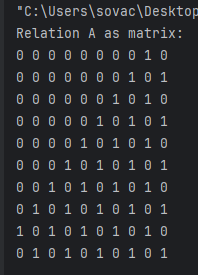
\includegraphics[width=50mm]{images/a_print.png}
			\caption{Матрица отношения A}
			\hfill
			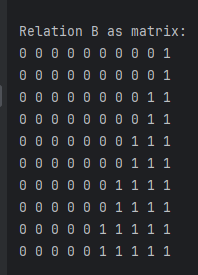
\includegraphics[width=50mm]{images/b_print.png}
			\caption{Матрица отношения B}
			\hfill
			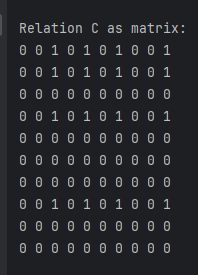
\includegraphics[width=50mm]{images/c_print.png}
			\caption{Матрица отношения C}
		\end{multicols}
	\end{figure}
	
	Легко убедиться, что матрицы отношений A, B, C аналогичны матрицам, которые мы составили в задании 1.1.
	
	\subsection{Задание 1.4}
	\label{subpart1_4}
	
	{\bf Текст задания:} Программно реализовать операции над отношениями.
	
	Напишем функции, реализующие операции сравнения отношений (проверка на включение, равенство, строгое включение), операции, аналогичные операциям над множествами (пересечение, объединение, разность, симметрическая разность, дополнение) и операции, не определенные для множеств (обращение, композиция, степень отношения). Здесь стоит заметить, что, поскольку  строки бинарной матрицы представлены целыми числами, с помощью побитовых операций их можно в одно действие сравнить, поняв, какие элементы встречаются только в одной, в обеих или ни в одной из матриц. Таким образом, многие операции можно реализовать без использования вложенных циклов.
	
	\lstinputlisting{../bin_relations/bin_relations_operations.c} 
	
	\subsection{Задание 1.5}
	\label{subpart1_5}
	
	{\bf Текст задания:} Написать программу, вычисляющую значение выражения (<<Варианты заданий>>, пункт {\bf б)}) и вычислить его при заданных отношениях (<<Варианты заданий>>, пункт {\bf a)}).
	
	Теперь, когда основные операции над отношениями реализованы программно, нам не составит труда вычислить значение выражения и вывести на экран отношение D. Для этого в соответствующей функции надо лишь в нужном порядке выполнить все операции (иногда сохраняя промежуточный результат в отдельных переменных для удобочитаемости) и вернуть окончательный результат вычислений. В теле функции main мы сначала вычисляем отношения A, B, C с помощью функций, написанных для решения задания 1.3, а потом вызываем функцию для вычисления отношения D, передавая отношения A, B, C как аргументы. Полученное отношение можно вывести на экран как в виде матрицы, так и в виде перечисления упорядоченных пар.
	
	\lstinputlisting{../bin_relations/main2.c} 
	\newpage
	
	\begin{figure}[h]
		\noindent\centering{
			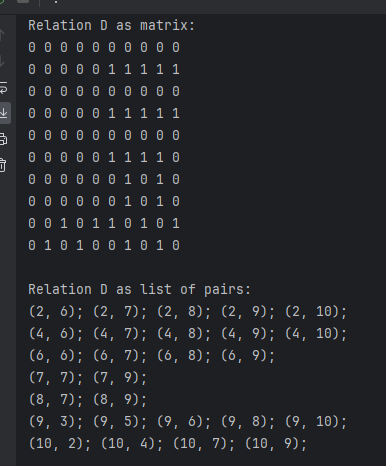
\includegraphics[width=100mm]{images/d_print.png}
			\caption{Вывод значения выражения D в двух формах}
		}
	\end{figure}
	
	Матрица отношения D соответствует графику, который мы построили в задании 1.2.
	\newpage
	
	\section{Часть 2. Свойства отношений}
	\subsection{Задание 2.1}
	\label{subpart2_1}
	{\bf Текст задания:} Определить основные и производные свойства отношений (<<Варианты заданий>>, пункт {\bf а)}).
	
	Определим основные свойства отношения $A$, для удобства снова приведя его матрицу: 

	\begin{tabular} {c c c c c c c c c c}
		0 & 0 & 0 & 0 & 0 & 0 & 0 & 0 & 1 & 0 \\
		0 & 0 & 0 & 0 & 0 & 0 & 0 & 1 & 0 & 1 \\
		0 & 0 & 0 & 0 & 0 & 0 & 1 & 0 & 1 & 0 \\
		0 & 0 & 0 & 0 & 0 & 1 & 0 & 1 & 0 & 1 \\
		0 & 0 & 0 & 0 & 1 & 0 & 1 & 0 & 1 & 0 \\
		0 & 0 & 0 & 1 & 0 & 1 & 0 & 1 & 0 & 1 \\
		0 & 0 & 1 & 0 & 1 & 0 & 1 & 0 & 1 & 0 \\
		0 & 1 & 0 & 1 & 0 & 1 & 0 & 1 & 0 & 1 \\
		1 & 0 & 1 & 0 & 1 & 0 & 1 & 0 & 1 & 0 \\
		0 & 1 & 0 & 1 & 0 & 1 & 0 & 1 & 0 & 1 \\
	\end{tabular}
	
	Анализируя эту матрицу, мы можем сказать, что:
	\begin{itemize}
		\item{Отношение $A$ {\bf не является ни рефлексивным, ни антирефлексивным}; мы ясно видим, что главная диагональ матрицы содержит как нули, так и единицы. К примеру, рефлексивным отношение $A$ не является хотя бы потому, что в него не входит пара $(1, 1)$, а антирефлексивным не является, потому что в него входит пара $(5, 5)$.}
		\item{Отношение $A$ {\bf является симметричным}; это можно как проследить в самой матрице, так и принять как следствие из факта, что вхождение или невхождение пары в отношение определяется суммой элементов, которая не зависит от их порядка. Очевидно, что если отношение $A$ является симметричным, то {\bf антисимметричным} оно точно {\bf не является}.}
		\item{Отношение $A$ {\bf не является ни транзитивным, ни антитранзитивным}. К примеру, транзитивным отношение $A$ не является хотя бы потому, что в него входят пары $(1, 9)$ и $(9, 3)$, но не входит пара $(1, 3)$. Антитранзитивным оно также не является хотя бы потому, что в него входят пары $(6, 8)$ и $(8, 4)$, а также пара $(6, 4)$.}
		\item{Отношение $A$ {\bf не является полным}, хотя бы потому, что в нее не входит ни пара $(1, 2)$, ни пара $(2, 1)$.}
	\end{itemize}
	
	Поскольку отношение $A$ не рефлексивно, его уже {\bf нельзя} назвать {\bf толерантным и эквивалентным}, а поскольку оно не является антисимметричным, то оно {\bf не обладает свойством порядка} и его частными случаями (свойствами {\bf нестрогого порядка, строгого порядка, линейного порядка, нестрогого линейного и строгого линейного порядка}).  
	\newpage
	
	Проделаем то же с отношением $B$, матрица которого выглядит так: 
	
	\begin{tabular} {c c c c c c c c c c}
		0 & 0 & 0 & 0 & 0 & 0 & 0 & 0 & 0 & 1 \\
		0 & 0 & 0 & 0 & 0 & 0 & 0 & 0 & 0 & 1 \\
		0 & 0 & 0 & 0 & 0 & 0 & 0 & 0 & 1 & 1 \\
		0 & 0 & 0 & 0 & 0 & 0 & 0 & 0 & 1 & 1 \\
		0 & 0 & 0 & 0 & 0 & 0 & 0 & 1 & 1 & 1 \\
		0 & 0 & 0 & 0 & 0 & 0 & 0 & 1 & 1 & 1 \\
		0 & 0 & 0 & 0 & 0 & 0 & 1 & 1 & 1 & 1 \\
		0 & 0 & 0 & 0 & 0 & 0 & 1 & 1 & 1 & 1 \\
		0 & 0 & 0 & 0 & 0 & 1 & 1 & 1 & 1 & 1 \\
		0 & 0 & 0 & 0 & 0 & 1 & 1 & 1 & 1 & 1 \\
	\end{tabular}
	
	Анализируя эту матрицу, мы можем сказать, что:
	\begin{itemize}
		\item{Отношение $B$ {\bf не является ни рефлексивным, ни антирефлексивным}; главная диагональ матрицы содержит как нули, так и единицы. К примеру, рефлексивным отношение $B$ не является хотя бы потому, что в него не входит пара $(1, 1)$, а антирефлексивным не является, потому что в него входит пара $(7, 7)$.}
		\item{Отношение $B$ {\bf не является ни симметричным, ни антисимметричным}. К примеру, его нельзя назвать симметричным хотя бы потому, что в него входит пара $(3, 9)$, но не входит пара $(9, 3)$. Антисимметричным его нельзя назвать хотя бы потому, что в него входят одновременно пары $(7, 9)$ и $(9, 7)$.}
		\item{Отношение $B$ {\bf не является ни транзитивным, ни антитранзитивным}. К примеру, транзитивным отношение $B$ не является хотя бы потому, что в него входят пары $(3, 9)$ и $(9, 7)$, но не входит пара $(3, 7)$. Антитранзитивным оно также не является хотя бы потому, что в него входят пары $(7, 8)$ и $(8, 10)$, а также пара $(7, 10)$.}
		\item{Отношение $B$ {\bf не является полным} хотя бы потому, что в нее не входит ни пара $(7, 3)$, ни пара $(3, 7)$.}
	\end{itemize}
	
	Поскольку отношение $B$ не рефлексивно, его уже {\bf нельзя} назвать {\bf толерантным и эквивалентным}, а поскольку оно не является антисимметричным, то оно {\bf не обладает} свойством {\bf порядка} и его частными случаями (свойствами {\bf нестрогого порядка, строгого порядка, линейного порядка, нестрогого линейного и строгого линейного порядка}). 
	
	Наконец, перейдем к отношению $C$, матрица которого выглядит так: 
	
	\begin{tabular} {c c c c c c c c c c}
		0 & 0 & 1 & 0 & 1 & 0 & 1 & 0 & 0 & 1 \\
		0 & 0 & 1 & 0 & 1 & 0 & 1 & 0 & 0 & 1 \\
		0 & 0 & 0 & 0 & 0 & 0 & 0 & 0 & 0 & 0 \\
		0 & 0 & 1 & 0 & 1 & 0 & 1 & 0 & 0 & 1 \\
		0 & 0 & 0 & 0 & 0 & 0 & 0 & 0 & 0 & 0 \\
		0 & 0 & 0 & 0 & 0 & 0 & 0 & 0 & 0 & 0 \\
		0 & 0 & 0 & 0 & 0 & 0 & 0 & 0 & 0 & 0 \\
		0 & 0 & 1 & 0 & 1 & 0 & 1 & 0 & 0 & 1 \\
		0 & 0 & 0 & 0 & 0 & 0 & 0 & 0 & 0 & 0 \\
		0 & 0 & 0 & 0 & 0 & 0 & 0 & 0 & 0 & 0 \\
	\end{tabular}
	
	Анализируя эту матрицу, мы можем сказать, что:
	\begin{itemize}
		\item{Отношение $C$ {\bf не является рефлексивным} уже потому, что в него не входит пара $(1, 1)$. Но это отношение {\bf является антирефлексивным}: главная диагональ матрицы содержит только нули, поскольку это отношение образовано декартовым произведением непересекающихся множеств, и в нем не может быть пар вида $(x, x)$.}
		\item{Отношение $C$ {\bf не является симметричным} уже потому, что в него входит пара $(1, 3)$, но не входит пара $(1, 3)$. Однако это отношение {\bf является антисимметричным}; это можно как проследить в самой матрице, так и принять как следствие из факта, что отношение образовано декартовым произведением непересекающихся множеств (обозначим их как $X$ и $Y$). Уже поэтому в отношение не могут входить одновременно пары $(x, y)$ и $(y, x)$, поскольку если элемент x принадлежит множеству $X$, он не будет входить в множество $Y$.}
		\item{Снова обратимся к тому факту, что отношение $C$ образовано декартовым произведением неких непересекающихся множеств $X$ и $Y$. Если в отношение входит пара вида $(x, z)$, то справедливо утверждение, что $z \in Y$, соответственно, $z \notin X$ и пара вида $(z, y)$ не может входить в отношение. Получается, в отношении $C$, не существует двух пар вида $(x, z)$ и $(z, y)$. Для любой тройки элементов $x, y, z$ в транзитивном отношении справедливо следствие $xRz \& zRy \to xRy$; а в антитранзитивном --- следствие $xRz \& zRy \to \overline{xRy}$. Но для любой тройки элементов в отношении $C$ конъюнкция $xRz \& zRy$ будет ложной, и любое следствие из нее будет истинным. Соотвественно, выполняются сразу оба условия, и отношение $C$ {\bf одновременно и транзитивно, и антитранзитивно}.}
		\item{Отношение $C$ {\bf не является полным}, хотя бы потому, что в нее не входит ни пара $(2, 4)$, ни пара $(4, 2)$.}
	\end{itemize}
	
	Поскольку отношение $C$ не рефлексивно, его уже {\bf нельзя} назвать {\bf толерантным и эквивалентным}. Оно {\bf обладает свойством порядка} (антисимметрично и транзитивно), при этом {\bf не обладает свойством нестрогого порядка} (так как не рефлексивно), но {\bf обладает свойством строгого порядка} (антирефлексивно). Оно {\bf не обладает свойством линейного порядка} (поскольку не является полным) и его частными случаями (свойствами {\bf нестрогого линейного и строгого линейного порядка}). 
	
	\subsection{Задание 2.2}
	\label{subpart2_2}
	{\bf Текст задания:} Для каждого основного свойства написать функцию, которая определяет, обладает ли этим свойством заданное отношение. Если отношение не обладает свойством, то функция должна дать этому объяснение.
	
	Для каждого основного свойства отношений (рефлексивности, антирефлексивности, симметричности, антисимметричности, транзитивности, антитранзитивности, полноты) напишем функции, определяющие, обладает ли отношение этим свойством. Если отношение обладает этим свойством, на экран выводится сообщение об этом; если отношение им не обладает, то сообщение об этом также будет содержать пару или пары, вхождение или невхождение которых в отношение доказывает это. Однако все эти функции, помимо вывода, возвращают соответствующее булево значение (<<истину>>, если отношение обладает данным свойством, и <<ложь>>, если не обладает) --- его можно сохранить в переменной и использовать в программе в дальнейшем. Пример этого --- последняя функций файла, которая вызывает все функции для основным свойств, сохраняя булевы значения в отдельных переменных и используя их для определения производных свойств. При этом для производных свойств сообщения выводятся только тогда, когда отношение обладает ими, а если оно не обладает некоторым производным свойством, то это свойство не упоминается. Впрочем, сообщение об отсутствии производных свойств выводится в эстетических целях.
	
	\lstinputlisting{../bin_relations/bin_relations_properties.c}
	
	\subsection{Задание 2.3}
	\label{subpart2_3}
	{\bf Текст задания:} 2.3. Написать программу, определяющую свойства отношения и определить свойства отношений (<<Варианты заданий>>, пункт {\bf а)}).
	
	Учитывая что в задании 2.2 мы задали функцию, выводящую на экран информацию о всех основных и производных свойствах отношения,  текущее задание сводится к тому, чтобы вызвать ее для каждого из отношений $A$, $B$, $C$.
	
	\lstinputlisting{../bin_relations/main3.c}
	
	\begin{figure}[h]
		\noindent\centering{
			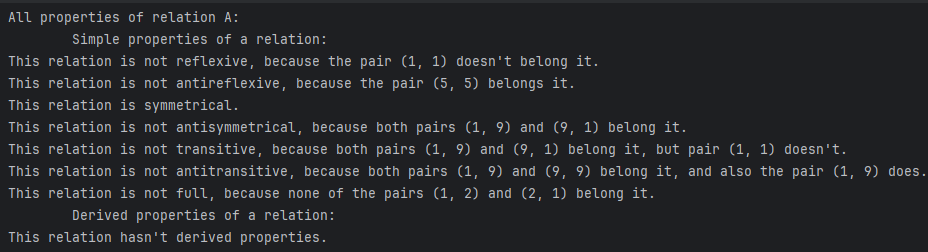
\includegraphics[width=170mm]{images/a_properties.png}
			\caption{Вывод свойств отношения A}
		}
		\end{figure}
	\newpage

\begin{figure}[h]
	\noindent\centering{
		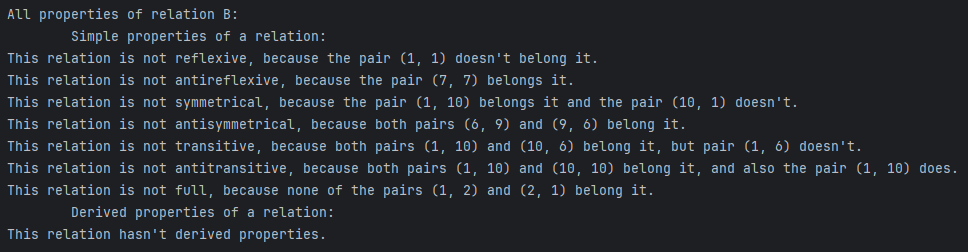
\includegraphics[width=170mm]{images/b_properties.png}
		\caption{Вывод свойств отношения B}

		}
	\end{figure}

	\begin{figure}[h]
		\noindent\centering{
			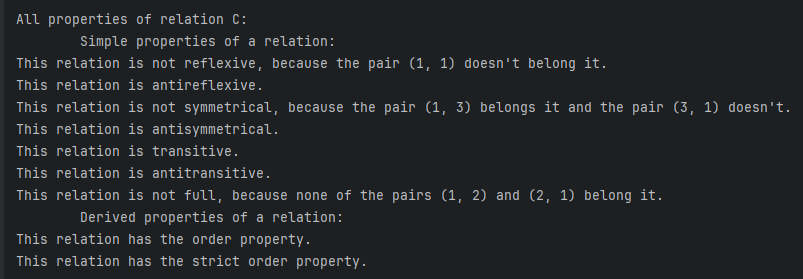
\includegraphics[width=170mm]{images/c_properties.png}
			\caption{Вывод свойств отношения C}
		}
	\end{figure}
		
	Выведенные на экран сообщения соответствуют умозаключениям, сделанным в задании 2.1.
	
	{\bf Вывод:} бинарное отношение --- частный случай бинарного соответствия, подмножество квадрата некоторого множества на само себя. Гораздо чаще приходится работать с бинарными отношениями, чем с бинарными соответствиями: отношения позволяют обозначить связи между элементами одного множества --- соответственно, между элементами, имеющими одинаковую природу. На основе уже существующих отношений можно создавать новые, отображающие более сложные связи; для этого используются операции над отношениями, как аналогичные операциям над множествами, так и не определенные для них. Сами отношения обладают характеристиками, наиболее важные из которых имеют отдельные названия и называются основными свойствами; производные свойства являются комбинацией основных. И в ходе выполнения этой лабораторной работы мы как научились вручную выполнять операции над отношениями и определять их свойства, так и реализовали функции для быстрого автоматизированного вычисления выражений с отношениями и определения их свойств.
	
\end{document}